\chapter{البلورات \texorpdfstring{\babelsublr{(2)}}{(2)}: الأجسام الصلبة الأيونية والتساهمية والجزيئية}\label{ch:b1:crystals-ionic-covalent}

ملح الطعام إذا سُحق يتكسّر إلى مكعبات دقيقة؛ والألماس أصلد المواد
الطبيعية، أما الغرافيت، المكوّن من ذرات الكربون نفسها، فطري
بما يكفي للكتابة به؛ والجليد يطفو على الماء. كلها بلورات، لكن
جسيماتها متماسكة بطرائق مختلفة: الأيونات بالتجاذب الكهربائي
الساكن، والذرات \omterm{def:b1:lewis-resonance-vsepr:lewis}{بالروابط التساهمية}، والجزيئات بالقوى
بين الجزيئية في \cref{ch:b1:intermolecular-forces-solvents}. يطبّق هذا الفصل
هندسة الخلية التي عرضها الفصل السابق على هذه العائلات الثلاث
من الأجسام الصلبة، ويفسّر، انطلاقًا من أحجام الأيونات، لماذا يتخذ كلوريد الصوديوم
وكلوريد السيزيوم بنيتين مختلفتين.

\begin{recall}
عُرّفت \omterm{def:b1:crystals-metals:multiplicity}{تعددية} الخلية \omterm{def:b1:crystals-metals:coordination}{وعدد التناسق} \omterm{def:b1:crystals-metals:compactness}{والاكتناز}، \omterm{def:b1:crystals-metals:site}{والمواقع
الثمانية الأوجه} والرباعية الأوجه \omterm{def:b1:crystals-metals:lattice}{لشبكة} \omterm{def:b1:crystals-metals:packings}{المكعب الممركز الأوجه}، في
\cref{ch:b1:crystals-metals}؛ والكتلة الحجمية \omterm{def:b1:crystals-metals:crystal}{للبلورة} هي
$\rho = ZM/(N_A V)$ (\cref{prop:b1:crystals-metals:density}). وقد قُدّمت أنصاف
الأقطار الأيونية في \cref{def:b1:periodicity:radius}.
\end{recall}

\section{البلورات الأيونية ونسب أنصاف الأقطار}

\begin{definition}[البلورة الأيونية]\label{def:b1:crystals-ionic-covalent:ionic-crystal}
\emph{البلورة الأيونية}\index{بلورة أيونية} \omterm{def:b1:crystals-metals:crystal}{بلورة} من كاتيونات
وأنيونات متماسكة بالتجاذب الكهربائي الساكن. كل أيون محاط
بأيونات معاكسة الشحنة؛ \omterm{def:b1:crystals-metals:crystal}{والبلورة} متعادلة كهربائيًا، فتكون
أعداد الكاتيونات والأنيونات في الخلية بنسبة الصيغة.
\end{definition}

\begin{proposition}[خواص البلورات الأيونية]\label{prop:b1:crystals-ionic-covalent:ionic-properties}
البلورات الأيونية صلدة لكنها هشة (فانزلاق طبقة واحدة يضع أيونات
من الإشارة نفسها وجهًا لوجه، فتنفلق \omterm{def:b1:crystals-metals:crystal}{البلورة})، ودرجات انصهارها
عالية، ولا توصل التيار وهي صلبة لكنها توصله منصهرة أو مذابة،
وتذوب في \omterm{def:b1:intermolecular-forces-solvents:solvent-classes}{المذيبات القطبية} العالية السماحية.
\end{proposition}
\admitted

\begin{definition}[نسبة أنصاف الأقطار]\label{def:b1:crystals-ionic-covalent:radius-ratio}
في \omterm{def:b1:crystals-ionic-covalent:ionic-crystal}{بلورة أيونية} من كاتيون نصف قطره $r_+$ وأنيون نصف قطره
$r_-$، تكون \emph{نسبة أنصاف الأقطار}\index{نسبة أنصاف الأقطار} $x = r_+/r_-$
(وعادةً $x < 1$، لأن الكاتيونات أصغر من الأنيونات).
\end{definition}

\begin{proposition}[قاعدة نسبة أنصاف الأقطار]\label{prop:b1:crystals-ionic-covalent:rule}
في نموذج الكرات الصلبة، لا تستقر البنية التي يمسّ فيها كل كاتيون $n$
أنيونًا إلا إذا لم تتماس الأنيونات فيما بينها، وهذا
يقتضي أن تفوق $x$ حدًا تفرضه الهندسة: $x \ge \sqrt3 - 1
\approx 0.732$ لثمانية جيران (مكعب)، و$x \ge \sqrt2 - 1 \approx 0.414$
لستة (ثماني أوجه)، و$x \ge \sqrt{3/2} - 1 \approx 0.225$ لأربعة
(رباعي أوجه). والبنية المتخذة هي ذات أعلى تناسق
تسمح به $x$.
\end{proposition}

\begin{proof}
يستقر الكاتيون في الفجوة بين $n$ أنيونًا تمسّه. وعند
الحد تتماس الأنيونات أيضًا فيما بينها. المكعب: الأنيونات على
رؤوس مكعب طول حرفه $2r_-$ والكاتيون في مركزه، فيكون $r_+ +
r_- = \sqrt3\,r_-$. ثماني الأوجه: أربعة أنيونات في مربع طول ضلعه $2r_-$،
والكاتيون في مركزه، $r_+ + r_- = \sqrt2\,r_-$. رباعي الأوجه:
الأنيونات على رؤوس متناوبة لمكعب طول حرفه $\sqrt2\,r_-$، والكاتيون في
المركز، $r_+ + r_- = \frac{\sqrt3}{2}\sqrt2\,r_- = \sqrt{3/2}\,r_-$.
وبالقسمة على $r_-$ نحصل على الحدود. وتحت الحد يتخلخل الكاتيون في
فجوة أوسع منه: فتتنافر الأنيونات دون أن يزداد التجاذب،
فيُفضَّل تناسق أدنى بفجوة أصغر.
\end{proof}

\begin{omfigure}
\begin{tikzpicture}[font=\small, >={Stealth}]
  \draw[->, thick] (0,0) -- (12.4,0) node[right] {$x = r_+/r_-$};
  \foreach \x/\l in {0/0, 2.7/0.225, 4.97/0.414, 8.78/0.732, 12/1} {
    \draw (\x,0.12) -- (\x,-0.12) node[below] {\l};
  }
  \fill[omDef!15] (2.7,0.2) rectangle (4.97,1.0);
  \fill[omProp!15] (4.97,0.2) rectangle (8.78,1.0);
  \fill[omThm!15] (8.78,0.2) rectangle (12,1.0);
  \node[align=center] at (3.83,0.6) {4: ZnS};
  \node[align=center] at (6.87,0.6) {6: NaCl};
  \node[align=center] at (10.4,0.6) {8: CsCl};
  \foreach \x/\l in {3.91/\ce{ZnS}, 6.76/\ce{NaCl}, 10.08/\ce{RbCl}, 11.54/\ce{CsCl}} {
    \draw[omExo, thick] (\x,-0.55) -- (\x,-0.95);
    \node[below, omExo] at (\x,-0.95) {\l};
  }
\end{tikzpicture}

{\small قاعدة \omterm{def:b1:crystals-ionic-covalent:radius-ratio}{نسبة أنصاف الأقطار}: عدد تناسق الكاتيون الذي
تسمح به $x$، والنسب المقيسة لأربعة أملاح (أنصاف أقطار شانون).
فكلوريد الروبيديوم، عند 0.84، ينبغي أن يكون من نمط \ce{CsCl} لكنه يتخذ
نمط \ce{NaCl}: فالقاعدة دليل، لا قانون
(\cref{exo:b1:crystals-ionic-covalent:12}).}
% ledger: rion:Zn2+IV, rion:S2-VI, rion:Na+VI, rion:Cl-VI, rion:Rb+VI,
% rion:Cs+VIII
\end{omfigure}

\section{أربعة أنماط بنيوية}

\begin{definition}[الأنماط البنيوية]\label{def:b1:crystals-ionic-covalent:structure-type}
تُصنَّف البلورات الأيونية في أنماط بنيوية قليلة، يسمّى كل منها
باسم مركب ممثل له:
\begin{itemize}
  \item \emph{نمط كلوريد السيزيوم}\index{نمط كلوريد السيزيوم}: الأنيونات
        على رؤوس مكعب، والكاتيون في مركزه (8:8)؛
  \item \emph{نمط الملح الصخري}\index{نمط الملح الصخري} (نمط كلوريد
        الصوديوم): الأنيونات على \omterm{def:b1:crystals-metals:lattice}{شبكة} مكعبة ممركزة الأوجه، والكاتيونات في كل مواقعها
        الثمانية الأوجه (6:6)؛
  \item \emph{نمط بلندة الزنك}\index{نمط بلندة الزنك}: الأنيونات على
        \omterm{def:b1:crystals-metals:lattice}{شبكة} مكعبة ممركزة الأوجه، والكاتيونات في نصف مواقعها الرباعية الأوجه، موقع من كل اثنين
        بالتناوب (4:4)؛
  \item \emph{نمط الفلوريت}\index{نمط الفلوريت}: الكاتيونات على
        \omterm{def:b1:crystals-metals:lattice}{شبكة} مكعبة ممركزة الأوجه، والأنيونات في كل مواقعها الرباعية الأوجه (8:4)، والصيغة
        \ce{MX2}؛ وفي \emph{نمط الفلوريت المعكوس}\index{نمط الفلوريت المعكوس}
        تتبادل الأدوار (\ce{Li2O}، 4:8).
\end{itemize}
ويعطي زوج الأعداد تناسق الكاتيون وتناسق
الأنيون.
\end{definition}

\begin{omfigure}
\tdplotsetmaincoords{60}{100}
\begin{tikzpicture}[tdplot_main_coords, font=\small]
  \pic {omcubeo={3}};
    \node[aX={green!55!black}{6.5mm}] at (0,0,0) {};
  \node[aX={violet!70}{3.8mm}] at (0,1.5,0) {};
  \node[aX={green!55!black}{6.5mm}] at (0,3,0) {};
  \node[aX={violet!70}{3.8mm}] at (0,0,1.5) {};
  \node[aX={green!55!black}{6.5mm}] at (0,1.5,1.5) {};
  \node[aX={violet!70}{3.8mm}] at (0,3,1.5) {};
  \node[aX={violet!70}{3.8mm}] at (1.5,0,0) {};
  \node[aX={green!55!black}{6.5mm}] at (0,0,3) {};
  \node[aX={green!55!black}{6.5mm}] at (1.5,1.5,0) {};
  \node[aX={violet!70}{3.8mm}] at (0,1.5,3) {};
  \node[aX={violet!70}{3.8mm}] at (1.5,3,0) {};
  \node[aX={green!55!black}{6.5mm}] at (0,3,3) {};
  \node[aX={green!55!black}{6.5mm}] at (1.5,0,1.5) {};
  \node[aX={violet!70}{3.8mm}] at (1.5,1.5,1.5) {};
  \node[aX={green!55!black}{6.5mm}] at (1.5,3,1.5) {};
  \node[aX={green!55!black}{6.5mm}] at (3,0,0) {};
  \node[aX={violet!70}{3.8mm}] at (1.5,0,3) {};
  \node[aX={violet!70}{3.8mm}] at (3,1.5,0) {};
  \node[aX={green!55!black}{6.5mm}] at (1.5,1.5,3) {};
  \node[aX={green!55!black}{6.5mm}] at (3,3,0) {};
  \node[aX={violet!70}{3.8mm}] at (1.5,3,3) {};
  \node[aX={violet!70}{3.8mm}] at (3,0,1.5) {};
  \node[aX={green!55!black}{6.5mm}] at (3,1.5,1.5) {};
  \node[aX={violet!70}{3.8mm}] at (3,3,1.5) {};
  \node[aX={green!55!black}{6.5mm}] at (3,0,3) {};
  \node[aX={violet!70}{3.8mm}] at (3,1.5,3) {};
  \node[aX={green!55!black}{6.5mm}] at (3,3,3) {};
  \node at (1.5,1.5,-1.75) {\foreignlanguage{arabic}{\ce{NaCl}، الملح الصخري}};
\end{tikzpicture}
\hspace{1cm}
\begin{tikzpicture}[tdplot_main_coords, font=\small]
  \pic {omcubeo={3}};
    \node[aX={green!55!black}{6.5mm}] at (0,0,0) {};
  \node[aX={green!55!black}{6.5mm}] at (0,3,0) {};
  \node[aX={green!55!black}{6.5mm}] at (0,0,3) {};
  \node[aX={green!55!black}{6.5mm}] at (0,3,3) {};
  \node[aX={blue!60}{7mm}] at (1.5,1.5,1.5) {};
  \node[aX={green!55!black}{6.5mm}] at (3,0,0) {};
  \node[aX={green!55!black}{6.5mm}] at (3,3,0) {};
  \node[aX={green!55!black}{6.5mm}] at (3,0,3) {};
  \node[aX={green!55!black}{6.5mm}] at (3,3,3) {};
  \node at (1.5,1.5,-1.75) {\ce{CsCl}};
\end{tikzpicture}

{\small يمينًا: خلية الملح الصخري، \ce{Cl-} (بالأخضر) على \omterm{def:b1:crystals-metals:lattice}{شبكة} مكعبة ممركزة الأوجه،
و\ce{Na+} (بالبنفسجي) في كل \omterm{def:b1:crystals-metals:site}{موقع ثماني الأوجه}. يسارًا: خلية كلوريد
السيزيوم، \ce{Cl-} على الرؤوس، و\ce{Cs+} (بالأزرق) في المركز. وقد رُسمت الأيونات
أصغر من حجمها عند التماس.}
\end{omfigure}

\begin{proposition}[نمطا الملح الصخري وكلوريد السيزيوم]\label{prop:b1:crystals-ionic-covalent:nacl-cscl}
في \omterm{def:b1:crystals-ionic-covalent:structure-type}{نمط الملح الصخري}، $Z = 4$ وحدات صيغة في كل خلية، وتتماس الأيونات
على امتداد الحرف، $a = 2(r_+ + r_-)$، وتقتضي البنية $\sqrt2 - 1
\le x$. وفي \omterm{def:b1:crystals-ionic-covalent:structure-type}{نمط كلوريد السيزيوم}، $Z = 1$، وتتماس الأيونات على امتداد
القطر الرئيسي، $a\sqrt3 = 2(r_+ + r_-)$، وتقتضي البنية
$x \ge \sqrt3 - 1$.
\end{proposition}

\begin{proof}
الملح الصخري: تُعدّ أنيونات \omterm{def:b1:crystals-metals:lattice}{الشبكة} الممركزة الأوجه $4$، والكاتيونات في \omterm{def:b1:crystals-metals:site}{المواقع
الثمانية الأوجه} الأربعة $1 + 12 \times \frac14 = 4$. وعلى امتداد الحرف يتتالى أنيون
وكاتيون وأنيون متماسة. ولا تتداخل الأنيونات
إذا حقق قطر الوجه، الذي يحوي ثلاثة أنيونات يتماس منها اثنان على
الأكثر، الشرط $a\sqrt2 \ge 4r_-$، أي $2(r_+ + r_-)\sqrt2 \ge
4r_-$، أو $x \ge \sqrt2 - 1$. كلوريد السيزيوم: $8 \times \frac18 = 1$
أنيون وكاتيون واحد؛ وعلى القطر الرئيسي أنيون وكاتيون وأنيون
متماسة؛ ولا تتداخل الأنيونات على امتداد الحرف إذا كان $a \ge 2r_-$، أي
$2(r_+ + r_-)/\sqrt3 \ge 2r_-$، أو $x \ge \sqrt3 - 1$.
\end{proof}

\begin{example}[كلوريد الصوديوم وكلوريد السيزيوم]\label{ex:b1:crystals-ionic-covalent:nacl}
لكلوريد الصوديوم $a = \qty{564.1}{pm}$: $r_+ + r_- = a/2 =
\qty{282.0}{pm}$، مقابل $102 + 181 = \qty{283}{pm}$ من أنصاف أقطار
شانون؛ و$x = 102/181 = 0.56$، في المجال الثماني الأوجه. وكتلته الحجمية
$\rho = 4 \times 58.44/(6.022 \times 10^{23} \times (5.641 \times
10^{-8})^3) = \qty{2.16}{g/cm^3}$، والمقيسة \qty{2.17}{g/cm^3}. ولكلوريد
السيزيوم $a = \qty{412.3}{pm}$: $r_+ + r_- = a\sqrt3/2 =
\qty{357.1}{pm}$، و$x = 174/181 = 0.96$، في المجال المكعب.
% ledger: lat:NaCl, rion:Na+VI, rion:Cl-VI, rho:NaCl, lat:CsCl,
% rion:Cs+VIII
\end{example}

\begin{omfigure}
\begin{minipage}[b]{0.31\linewidth}\centering
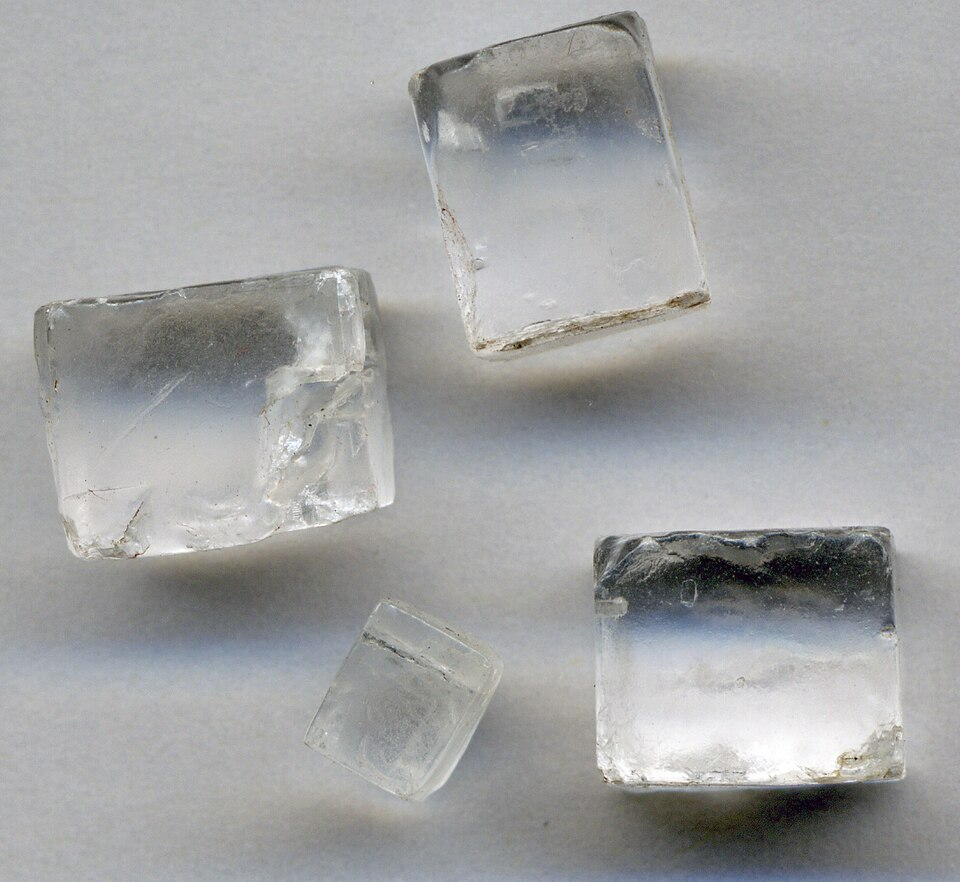
\includegraphics[width=\linewidth]{images/book2/halite.jpg}

{\small بلورات هاليت (ملح صخري). تصوير: جيمس سانت جون، CC BY 2.0.}
\end{minipage}\hfill
\begin{minipage}[b]{0.31\linewidth}\centering
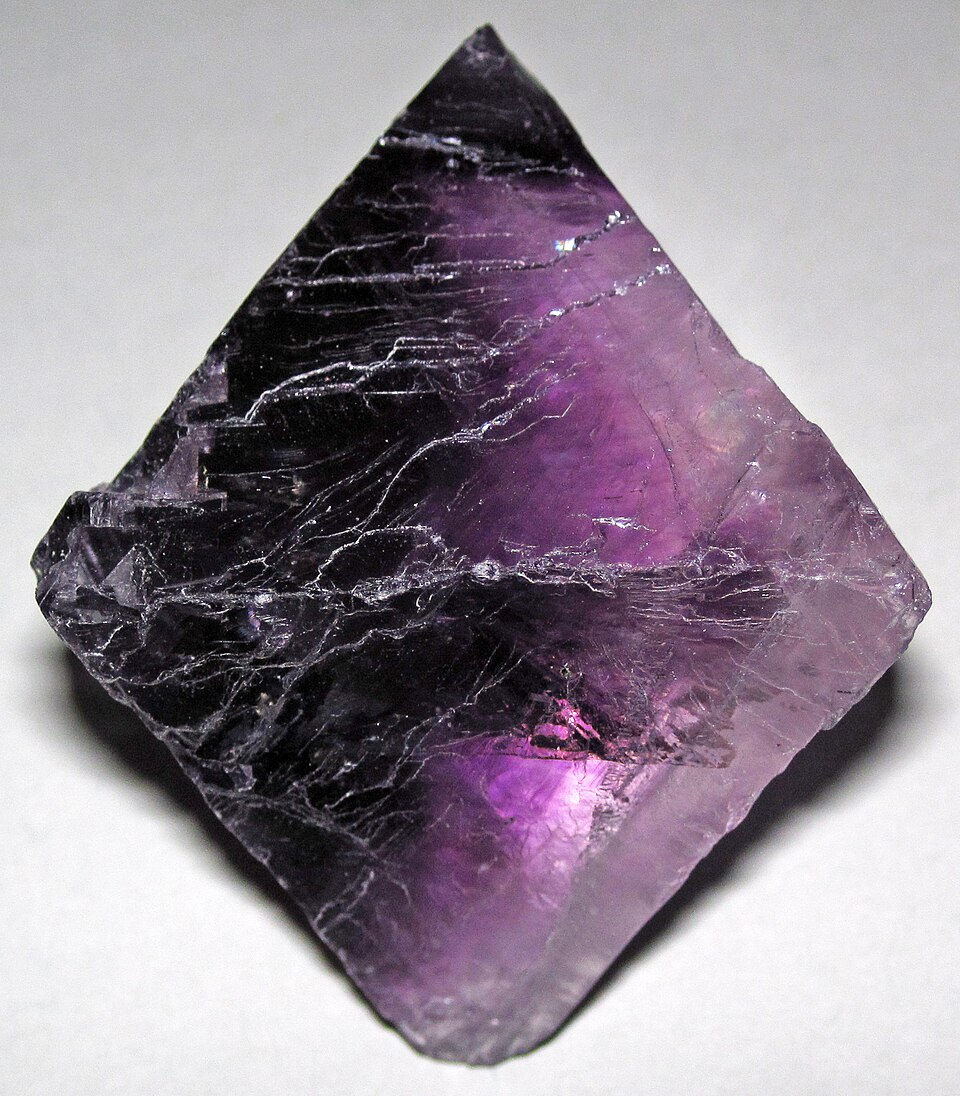
\includegraphics[width=0.85\linewidth]{images/book2/fluorite.jpg}

{\small الفلوريت، \ce{CaF2}. تصوير: جيمس سانت جون، CC BY 2.0.}
\end{minipage}\hfill
\begin{minipage}[b]{0.31\linewidth}\centering
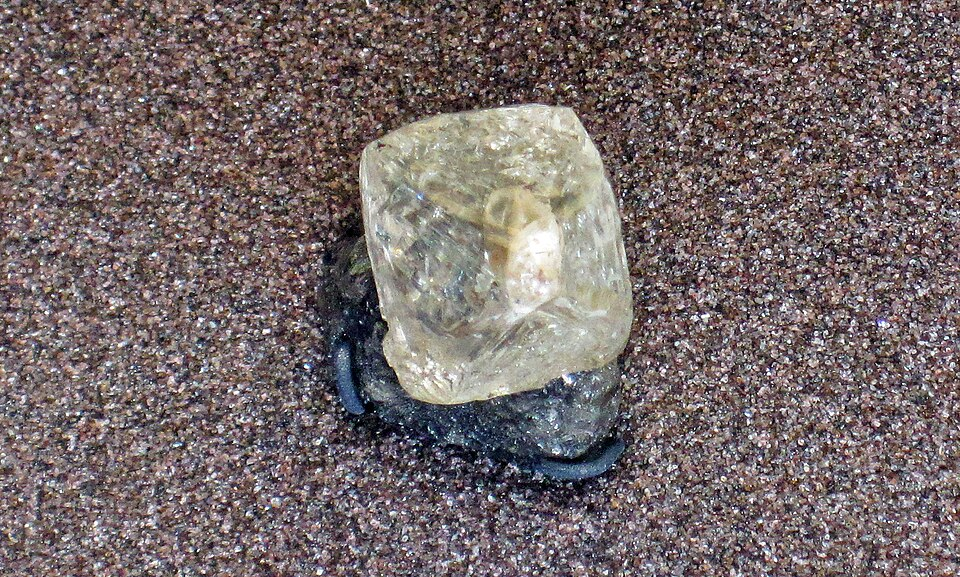
\includegraphics[width=\linewidth]{images/book2/diamond.jpg}

{\small ثماني أوجه خام من الألماس. تصوير: جيمس سانت جون، CC BY 2.0.}
\end{minipage}
\end{omfigure}

\begin{proposition}[نمطا بلندة الزنك والفلوريت]\label{prop:b1:crystals-ionic-covalent:zns-caf2}
في \omterm{def:b1:crystals-ionic-covalent:structure-type}{نمط بلندة الزنك}، $Z = 4$، وكل أيون محاط بأربعة من
النوع الآخر على رؤوس رباعي أوجه، وتتماس الأيونات على امتداد
ربع القطر الرئيسي: $a\sqrt3/4 = r_+ + r_-$. وفي \omterm{def:b1:crystals-ionic-covalent:structure-type}{نمط
الفلوريت}، $Z = 4$ وحدات \ce{CaF2}، ولكل كاتيون 8 جيران من الأنيونات (مكعب)،
ولكل أنيون 4 جيران من الكاتيونات (رباعي أوجه)، ومرة أخرى $a\sqrt3/4 =
r_+ + r_-$.
\end{proposition}

\begin{proof}
بلندة الزنك: 4 أنيونات على \omterm{def:b1:crystals-metals:lattice}{الشبكة} الممركزة الأوجه و4 كاتيونات في نصف \omterm{def:b1:crystals-metals:site}{المواقع
الرباعية الأوجه} الثمانية. \omterm{def:b1:crystals-metals:site}{والموقع الرباعي الأوجه} عند $(\frac a4,\frac a4,\frac a4)$
يقع على مسافة $\frac{a\sqrt3}{4}$ من أنيوناته الأربعة. الفلوريت: 4 كاتيونات
و8 أنيونات في كل \omterm{def:b1:crystals-metals:site}{المواقع الرباعية الأوجه}، بنسبة $1:2$. والأنيونات الثمانية داخل
الخلية تكوّن مكعبًا طول حرفه $a/2$، وفي مكعبات الأنيونات يقع
كاتيون في مركز مكعب من كل اثنين؛ ولكل أنيون جيرانه الأربعة من الكاتيونات
على مسافة $\frac{a\sqrt3}{4}$.
\end{proof}

\begin{omfigure}
\tdplotsetmaincoords{60}{100}
\begin{tikzpicture}[tdplot_main_coords, font=\small]
  \pic {omcubeo={3}};
  \begin{scope}[on background layer]
    \draw[black!45, line width=1.2pt] (0.75,0.75,2.25) -- (0,0,3) (0.75,0.75,2.25) -- (0,1.5,1.5) (0.75,0.75,2.25) -- (1.5,0,1.5) (0.75,0.75,2.25) -- (1.5,1.5,3) (0.75,2.25,0.75) -- (0,1.5,1.5) (0.75,2.25,0.75) -- (0,3,0) (0.75,2.25,0.75) -- (1.5,1.5,0) (0.75,2.25,0.75) -- (1.5,3,1.5) (2.25,0.75,0.75) -- (1.5,0,1.5) (2.25,0.75,0.75) -- (1.5,1.5,0) (2.25,0.75,0.75) -- (3,0,0) (2.25,0.75,0.75) -- (3,1.5,1.5) (2.25,2.25,2.25) -- (1.5,1.5,3) (2.25,2.25,2.25) -- (1.5,3,1.5) (2.25,2.25,2.25) -- (3,1.5,1.5) (2.25,2.25,2.25) -- (3,3,3);
  \end{scope}
    \node[aX={yellow!75!orange}{6mm}] at (0,0,0) {};
  \node[aX={yellow!75!orange}{6mm}] at (0,3,0) {};
  \node[aX={yellow!75!orange}{6mm}] at (0,1.5,1.5) {};
  \node[aX={gray!60}{3.6mm}] at (0.75,2.25,0.75) {};
  \node[aX={yellow!75!orange}{6mm}] at (0,0,3) {};
  \node[aX={yellow!75!orange}{6mm}] at (1.5,1.5,0) {};
  \node[aX={gray!60}{3.6mm}] at (0.75,0.75,2.25) {};
  \node[aX={yellow!75!orange}{6mm}] at (0,3,3) {};
  \node[aX={yellow!75!orange}{6mm}] at (1.5,0,1.5) {};
  \node[aX={gray!60}{3.6mm}] at (2.25,0.75,0.75) {};
  \node[aX={yellow!75!orange}{6mm}] at (1.5,3,1.5) {};
  \node[aX={yellow!75!orange}{6mm}] at (3,0,0) {};
  \node[aX={yellow!75!orange}{6mm}] at (1.5,1.5,3) {};
  \node[aX={yellow!75!orange}{6mm}] at (3,3,0) {};
  \node[aX={gray!60}{3.6mm}] at (2.25,2.25,2.25) {};
  \node[aX={yellow!75!orange}{6mm}] at (3,1.5,1.5) {};
  \node[aX={yellow!75!orange}{6mm}] at (3,0,3) {};
  \node[aX={yellow!75!orange}{6mm}] at (3,3,3) {};
  \node at (1.5,1.5,-1.75) {\foreignlanguage{arabic}{\ce{ZnS}، بلندة الزنك}};
\end{tikzpicture}
\hspace{1cm}
\begin{tikzpicture}[tdplot_main_coords, font=\small]
  \pic {omcubeo={3}};
    \node[aX={green!35!gray}{4.4mm}] at (0,0,0) {};
  \node[aX={green!35!gray}{4.4mm}] at (0,3,0) {};
  \node[aX={green!35!gray}{4.4mm}] at (0,1.5,1.5) {};
  \node[aX={green!45!yellow}{5.0mm}] at (0.75,0.75,0.75) {};
  \node[aX={green!45!yellow}{5.0mm}] at (0.75,2.25,0.75) {};
  \node[aX={green!35!gray}{4.4mm}] at (0,0,3) {};
  \node[aX={green!35!gray}{4.4mm}] at (1.5,1.5,0) {};
  \node[aX={green!45!yellow}{5.0mm}] at (0.75,0.75,2.25) {};
  \node[aX={green!35!gray}{4.4mm}] at (0,3,3) {};
  \node[aX={green!35!gray}{4.4mm}] at (1.5,0,1.5) {};
  \node[aX={green!45!yellow}{5.0mm}] at (0.75,2.25,2.25) {};
  \node[aX={green!45!yellow}{5.0mm}] at (2.25,0.75,0.75) {};
  \node[aX={green!35!gray}{4.4mm}] at (1.5,3,1.5) {};
  \node[aX={green!35!gray}{4.4mm}] at (3,0,0) {};
  \node[aX={green!45!yellow}{5.0mm}] at (2.25,2.25,0.75) {};
  \node[aX={green!35!gray}{4.4mm}] at (1.5,1.5,3) {};
  \node[aX={green!35!gray}{4.4mm}] at (3,3,0) {};
  \node[aX={green!45!yellow}{5.0mm}] at (2.25,0.75,2.25) {};
  \node[aX={green!45!yellow}{5.0mm}] at (2.25,2.25,2.25) {};
  \node[aX={green!35!gray}{4.4mm}] at (3,1.5,1.5) {};
  \node[aX={green!35!gray}{4.4mm}] at (3,0,3) {};
  \node[aX={green!35!gray}{4.4mm}] at (3,3,3) {};
  \node at (1.5,1.5,-1.75) {\foreignlanguage{arabic}{\ce{CaF2}، الفلوريت}};
\end{tikzpicture}

{\small يمينًا: بلندة الزنك، \ce{S^{2-}} (بالأصفر) على \omterm{def:b1:crystals-metals:lattice}{شبكة} مكعبة ممركزة الأوجه
و\ce{Zn^{2+}} (بالرمادي) في \omterm{def:b1:crystals-metals:site}{مواقع رباعية الأوجه} متناوبة، كل منها موصول بجيرانه
الأربعة. يسارًا: الفلوريت، \ce{Ca^{2+}} (بالرمادي المخضرّ) على \omterm{def:b1:crystals-metals:lattice}{شبكة} مكعبة
ممركزة الأوجه و\ce{F-} (بالأخضر الفاتح) في \omterm{def:b1:crystals-metals:site}{المواقع الرباعية الأوجه} الثمانية كلها.}
\end{omfigure}

\begin{example}[بلندة الزنك والفلوريت]\label{ex:b1:crystals-ionic-covalent:zns}
لبلندة الزنك $a = \qty{540.9}{pm}$: $r_+ + r_- = a\sqrt3/4 =
\qty{234.2}{pm}$ (شانون: $60 + 184 = \qty{244}{pm}$، إذ لا يُجدوَل نصف قطر
الكبريتيد إلا لستة جيران)، و$x = 60/184 = 0.33$، في
المجال الرباعي الأوجه. وللفلوريت $a = \qty{546.3}{pm}$: $r_+ + r_- =
\qty{236.6}{pm}$ (شانون $112 + 131 = \qty{243}{pm}$)، و$x = 0.85$:
فالكاتيون يستقر في مكعب من 8 أنيونات، كما تقتضي القاعدة.
% ledger: lat:ZnS, rion:Zn2+IV, rion:S2-VI, lat:CaF2, rion:Ca2+VIII,
% rion:F-IV
\end{example}

\begin{method}[التنبؤ ببنية]\label{met:b1:crystals-ionic-covalent:predict}
للتنبؤ ببنية مركب أيوني \ce{MX} أو \ce{MX2}:
\begin{enumerate}
  \item احسب $x = r_+/r_-$ من أنصاف الأقطار المجدولة (للتناسق
        المتوقع)؛
  \item اقرأ تناسق الكاتيون من قاعدة \omterm{def:b1:crystals-ionic-covalent:radius-ratio}{نسبة أنصاف الأقطار}؛
  \item اختر النمط الذي له هذا التناسق والصيغة الصحيحة:
        \ce{MX} مع 8: \ce{CsCl}؛ ومع 6: \ce{NaCl}؛ ومع 4: بلندة الزنك؛
        و\ce{MX2} مع 8: الفلوريت؛
  \item تحقق بمقارنته بوسيط \omterm{def:b1:crystals-metals:lattice}{الشبكة} المقيس؛ وتذكّر أن
        الأيونات القابلة للاستقطاب (\ce{S^{2-}}، \ce{I-}) والكاتيونات الصغيرة المشحونة
        تعطي \omterm{def:b1:lewis-resonance-vsepr:lewis}{روابط تساهمية} جزئيًا، تخفق فيها القاعدة.
\end{enumerate}
\end{method}

\section{البلورات التساهمية}

\begin{definition}[البلورة التساهمية]\label{def:b1:crystals-ionic-covalent:covalent-crystal}
\emph{البلورة التساهمية}\index{بلورة تساهمية} (أو الجسم الصلب الشبكي)
\omterm{def:b1:crystals-metals:crystal}{بلورة} ترتبط فيها كل الذرات \omterm{def:b1:lewis-resonance-vsepr:lewis}{بروابط تساهمية} في جزيء
عملاق واحد: الألماس، والسيليكون، والكوارتز \ce{SiO2}. وفي \omterm{def:b1:crystals-metals:crystal}{البلورة} التساهمية
الطبقية مثل الغرافيت، لا تمتد \omterm{def:b1:crystals-metals:lattice}{الشبكة} التساهمية إلا في
مستويات، تتماسك فيما بينها \omterm{def:b1:intermolecular-forces-solvents:vdw}{بتآثرات فان دير فالس}.
\end{definition}

\begin{proposition}[بنية الألماس]\label{prop:b1:crystals-ionic-covalent:diamond}
في الألماس تشغل ذرات الكربون \omterm{def:b1:crystals-metals:lattice}{الشبكة} الممركزة الأوجه ونصف
مواقعها الرباعية الأوجه، كنوعي الأيونات في بلندة الزنك: $Z = 8$، وكل
كربون مرتبط بأربعة أخرى على رؤوس رباعي أوجه، على
المسافة $a\sqrt3/4$. ومن أجل كرات متماسة يكون \omterm{def:b1:crystals-metals:compactness}{الاكتناز}
\[
  C = \frac{\pi\sqrt3}{16} \approx 0.34 .
\]
\end{proposition}

\begin{proof}
$Z = 4 + 4 = 8$. والذرات المتجاورة متماسة: $2R = a\sqrt3/4$، فيكون $a =
8R/\sqrt3$ و$C = 8 \cdot \frac43\pi R^3/a^3 = \frac{32}{3}\pi R^3 \cdot
\frac{3\sqrt3}{512 R^3} = \frac{\pi\sqrt3}{16}$.
\end{proof}

\begin{omfigure}
\tdplotsetmaincoords{60}{100}
\begin{tikzpicture}[tdplot_main_coords, font=\small]
  \pic {omcubeo={3}};
  \begin{scope}[on background layer]
    \draw[black!55, line width=1.4pt] (0.75,0.75,2.25) -- (0,0,3) (0.75,0.75,2.25) -- (0,1.5,1.5) (0.75,0.75,2.25) -- (1.5,0,1.5) (0.75,0.75,2.25) -- (1.5,1.5,3) (0.75,2.25,0.75) -- (0,1.5,1.5) (0.75,2.25,0.75) -- (0,3,0) (0.75,2.25,0.75) -- (1.5,1.5,0) (0.75,2.25,0.75) -- (1.5,3,1.5) (2.25,0.75,0.75) -- (1.5,0,1.5) (2.25,0.75,0.75) -- (1.5,1.5,0) (2.25,0.75,0.75) -- (3,0,0) (2.25,0.75,0.75) -- (3,1.5,1.5) (2.25,2.25,2.25) -- (1.5,1.5,3) (2.25,2.25,2.25) -- (1.5,3,1.5) (2.25,2.25,2.25) -- (3,1.5,1.5) (2.25,2.25,2.25) -- (3,3,3);
  \end{scope}
  \node[aX={black!65}{3.6mm}] at (0,0,0) {};
  \node[aX={black!65}{3.6mm}] at (0,3,0) {};
  \node[aX={black!65}{3.6mm}] at (0,1.5,1.5) {};
  \node[aX={black!65}{3.6mm}] at (0.75,2.25,0.75) {};
  \node[aX={black!65}{3.6mm}] at (0,0,3) {};
  \node[aX={black!65}{3.6mm}] at (1.5,1.5,0) {};
  \node[aX={black!65}{3.6mm}] at (0.75,0.75,2.25) {};
  \node[aX={black!65}{3.6mm}] at (0,3,3) {};
  \node[aX={black!65}{3.6mm}] at (1.5,0,1.5) {};
  \node[aX={black!65}{3.6mm}] at (2.25,0.75,0.75) {};
  \node[aX={black!65}{3.6mm}] at (1.5,3,1.5) {};
  \node[aX={black!65}{3.6mm}] at (3,0,0) {};
  \node[aX={black!65}{3.6mm}] at (1.5,1.5,3) {};
  \node[aX={black!65}{3.6mm}] at (3,3,0) {};
  \node[aX={black!65}{3.6mm}] at (2.25,2.25,2.25) {};
  \node[aX={black!65}{3.6mm}] at (3,1.5,1.5) {};
  \node[aX={black!65}{3.6mm}] at (3,0,3) {};
  \node[aX={black!65}{3.6mm}] at (3,3,3) {};
  \node at (1.5,1.5,-1.75) {الألماس};
\end{tikzpicture}
\hspace{0.8cm}
\begin{tikzpicture}[font=\small, y={(0cm,0.45cm)}, z={(0cm,1cm)}, x={(1cm,0cm)}]
  % two honeycomb layers seen in perspective, ABAB stacking
  \foreach \zz/\dy/\col in {0/0/black!40, 1.7/0.82/black!80} {
    \foreach \i in {0,1,2} \foreach \j in {0,1} {
      \pgfmathsetmacro\cx{1.42*\i+0.71*\j}
      \pgfmathsetmacro\cy{1.23*\j+\dy}
      \foreach \k in {0,60,...,300} {
        \pgfmathsetmacro\ka{\k+60}
        \draw[\col, line width=1pt] ({\cx+0.82*cos(\k+30)},{\cy+0.82*sin(\k+30)},\zz)
          -- ({\cx+0.82*cos(\ka+30)},{\cy+0.82*sin(\ka+30)},\zz);
      }
    }
  }
  \draw[<->, omThm] (5.6,0.9,0) -- (5.6,0.9,1.7) node[midway, right] {\qty{335}{pm}};
  \node at (2.4,-1.6,0) {الغرافيت};
\end{tikzpicture}

{\small يمينًا: خلية الألماس، وكل كربون مرتبط بأربعة أخرى في
رباعي أوجه. يسارًا: الغرافيت، طبقات من السداسيات (C--C \qty{141.8}{pm}
داخل الطبقة) مكدّسة على بعد \qty{334.8}{pm} بعضها من بعض، تمسكها قوى لندن؛ وتتناوب
الطبقات وفق ABAB.}
% ledger: lat:C-graphite.a, lat:C-graphite.c (C-C = a/sqrt3; interlayer = c/2)
\end{omfigure}

\begin{example}[الألماس والسيليكون والغرافيت]\label{ex:b1:crystals-ionic-covalent:carbon}
للألماس $a = \qty{356.7}{pm}$: \ce{C-C} $= a\sqrt3/4 =
\qty{154.5}{pm}$، وهي الرابطة الأحادية في الإيثان، و$\rho =
\qty{3.52}{g/cm^3}$. وللسيليكون، ذي البنية نفسها مع $a =
\qty{543.1}{pm}$، \ce{Si-Si} $= \qty{235.2}{pm}$ و$\rho =
\qty{2.33}{g/cm^3}$ (والمقيسة 2.33). وفي الغرافيت كل كربون مرتبط
بثلاثة أخرى في مستوٍ على \qty{141.8}{pm}، وهي رتبة رابطة بين الواحد
والاثنين (رنين على امتداد الطبقة)، بينما تتباعد الطبقات
\qty{334.8}{pm}. فالألماس، الصلب في الأبعاد الثلاثة، أصلد المواد
الطبيعية وعازل؛ أما الغرافيت فينفلق بين طبقاته،
التي تنزلق بسهولة، ويوصل الكهرباء داخلها بفضل إلكترونات $\pi$
المتمركزة على امتداد الطبقة.
% ledger: lat:C-diamond, lat:Si, rho:Si, lat:C-graphite.a, lat:C-graphite.c,
% geo:C2H6.rCC
\end{example}

\begin{omfigure}
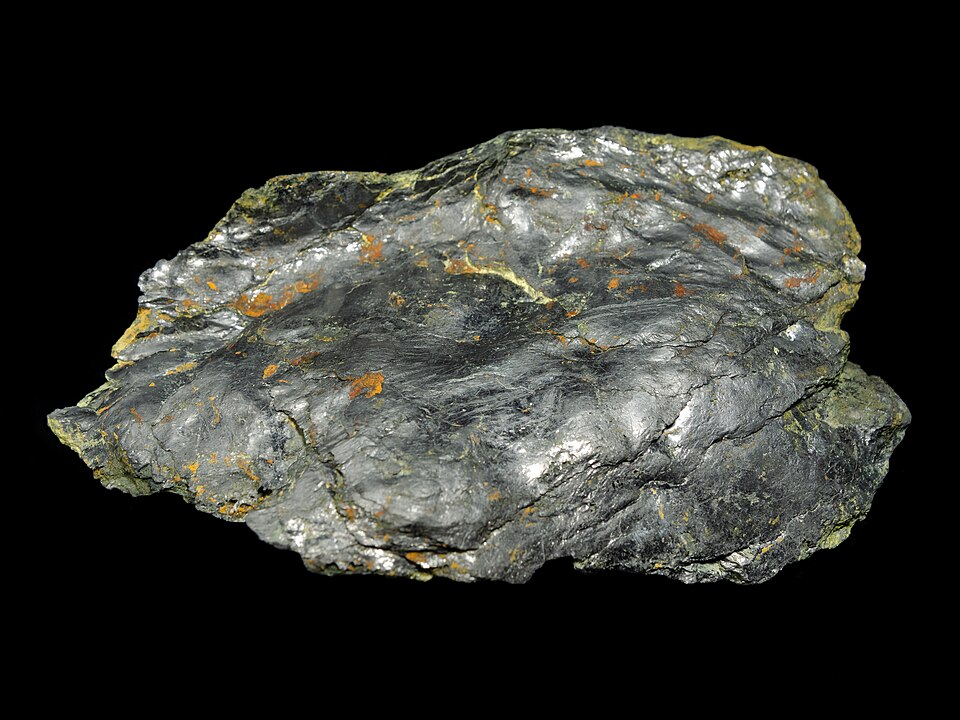
\includegraphics[width=0.36\linewidth]{images/book2/graphite.jpg}

{\small عيّنة من الغرافيت الطبيعي، ببريقها الفلزي. تصوير:
زبينيك بوريفال، CC BY-SA 4.0.}
\end{omfigure}

\section{البلورات الجزيئية}

\begin{definition}[البلورة الجزيئية]\label{def:b1:crystals-ionic-covalent:molecular-crystal}
\emph{البلورة الجزيئية}\index{بلورة جزيئية} \omterm{def:b1:crystals-metals:crystal}{بلورة} من
جزيئات متماسكة بالقوى بين الجزيئية --- \omterm{def:b1:intermolecular-forces-solvents:vdw}{تآثرات فان دير فالس}
و، إن أمكن، \omterm{def:b1:intermolecular-forces-solvents:hbond}{الروابط الهيدروجينية} --- بينما يحتفظ كل جزيء
بروابطه التساهمية: ثنائي اليود، والثلج الجاف \ce{CO2(s)}، والجليد، والسكر.
\end{definition}

\begin{proposition}[خواص البلورات الجزيئية]\label{prop:b1:crystals-ionic-covalent:molecular}
البلورات الجزيئية طرية وتنصهر أو تتسامى عند درجات حرارة منخفضة،
لأنه لا يُكسر فيها إلا قوى بين جزيئية ضعيفة؛ ولا توصل التيار.
\end{proposition}
\admitted

\begin{example}[الجليد]\label{ex:b1:crystals-ionic-covalent:ice}
في الجليد العادي يرتبط كل جزيء ماء \omterm{def:b1:intermolecular-forces-solvents:hbond}{بروابط هيدروجينية} بأربعة أخرى على
رؤوس رباعي أوجه: اثنان بذرتي هيدروجينه واثنان بزوجيه
الحرين. وهذه \omterm{def:b1:crystals-metals:lattice}{الشبكة} السداسية المفتوحة، التي تفرضها اتجاهات
\omterm{def:b1:intermolecular-forces-solvents:hbond}{الروابط الهيدروجينية}، تترك فراغًا كبيرًا: فالجليد أقل كثافة من الماء
السائل، الذي تنكسر فيه \omterm{def:b1:crystals-metals:lattice}{الشبكة} جزئيًا وتقترب
الجزيئات. ويظهر التناظر السداسي \omterm{def:b1:crystals-metals:lattice}{للشبكة} في الشكل السداسي
لبلورات الثلج.
\end{example}

\begin{omfigure}
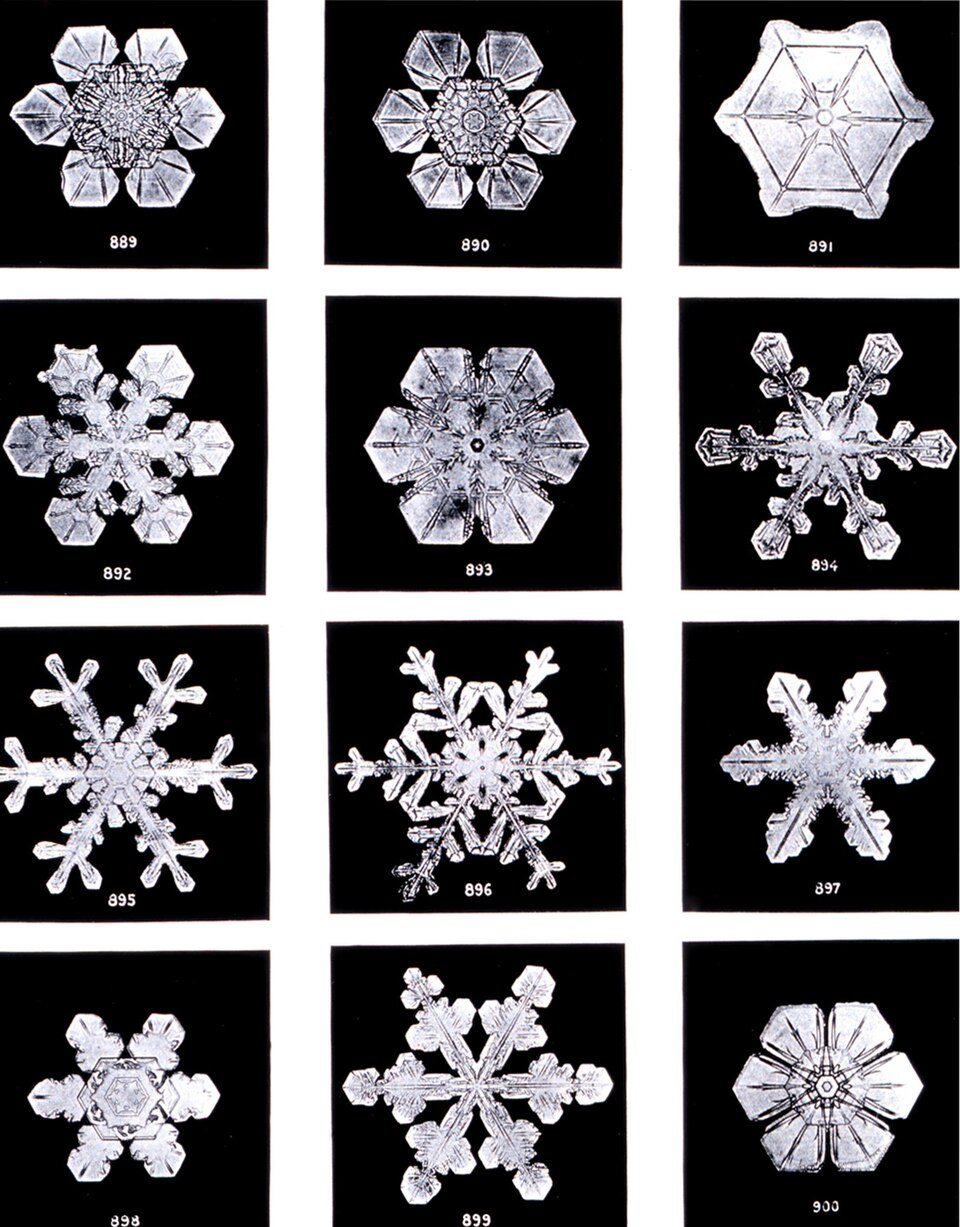
\includegraphics[width=0.38\linewidth]{images/book2/bentley-snowflakes.jpg}

{\small بلورات ثلج صوّرها ويلسون بنتلي نحو سنة 1902: لكل منها
تناظر سداسي، وهو أثر \omterm{def:b1:crystals-metals:lattice}{الشبكة} السداسية \omterm{def:b1:intermolecular-forces-solvents:hbond}{للروابط
الهيدروجينية} في الجليد. ملكية عامة.}
\end{omfigure}

\section{مقارنة الأنواع الأربعة من الأجسام الصلبة}

\begin{center}
\small
\begin{tabular}{lllll}
\hline
الجسم الصلب & الجسيمات & التماسك & الخواص & أمثلة \\
\hline
فلزي & كاتيونات، إلكترونات & \omterm{def:b1:crystals-metals:metallic-bond}{رابطة فلزية} & موصل، مطيل & \ce{Cu}، \ce{Fe}، \ce{Na} \\
أيوني & كاتيونات، أنيونات & كهربائي ساكن & صلد، هش، عازل & \ce{NaCl}، \ce{CaF2} \\
تساهمي & ذرات & \omterm{def:b1:lewis-resonance-vsepr:lewis}{روابط تساهمية} & صلد جدًا، عالي الانصهار & الألماس، \ce{SiO2} \\
جزيئي & جزيئات & فان دير فالس، روابط H & طري، منخفض الانصهار & \ce{I2}، الجليد \\
\hline
\end{tabular}
\end{center}

\begin{remark}[متصل]\label{rem:b1:crystals-ionic-covalent:continuum}
هذه الأصناف تجريدات. فلكبريتيد الزنك روابط أيونية جزئيًا
وتساهمية جزئيًا، ولهذا كانت مسافة كبريتيد--زنك فيه أقصر من
مجموع نصفي القطرين الأيونيين؛ والغرافيت تساهمي في طبقاته
وجزيئي بينها. ويبقى فرق \omterm{def:b1:periodicity:electronegativity}{الكهرسلبية}
(\cref{prop:b1:periodicity:en-trend}) هو الدليل: فكلما كبر كان
الجسم الصلب أكثر أيونية.
\end{remark}

\section{تمارين}

\begin{exercise}[$\star$]\label{exo:b1:crystals-ionic-covalent:1}
في خلية الملح الصخري، عُدّ الكاتيونات والأنيونات، وأعطِ
تناسق كل منها، وتحقق من احترام الصيغة \ce{NaCl}.
\end{exercise}

\begin{exercise}[$\star$]\label{exo:b1:crystals-ionic-covalent:2}
لكلوريد السيزيوم $a = \qty{412.3}{pm}$. احسب أقصر مسافة
\ce{Cs-Cl} وعدد وحدات الصيغة في كل خلية.
\end{exercise}

\begin{exercise}[$\star$]\label{exo:b1:crystals-ionic-covalent:3}
مستعملًا نصفي القطرين $r(\ce{Na+}) = \qty{102}{pm}$ و$r(\ce{Cl-}) =
\qty{181}{pm}$، احسب \omterm{def:b1:crystals-ionic-covalent:radius-ratio}{نسبة أنصاف الأقطار} في \ce{NaCl} وتنبأ
بتناسق الكاتيون.
\end{exercise}

\begin{exercise}[$\star$]\label{exo:b1:crystals-ionic-covalent:4}
صنّف إلى فلزي أو أيوني أو تساهمي أو جزيئي: النحاس، وكلوريد
الصوديوم، والألماس، وثنائي اليود، والكوارتز \ce{SiO2}، والجليد، وفلوريد الكالسيوم.
\end{exercise}

\begin{exercise}[$\star\star$]\label{exo:b1:crystals-ionic-covalent:5}
برهن على أن بنية الملح الصخري تقتضي $r_+/r_- \ge \sqrt2 - 1$.
\end{exercise}

\begin{exercise}[$\star\star$]\label{exo:b1:crystals-ionic-covalent:6}
احسب الكتلة الحجمية لكلوريد الصوديوم انطلاقًا من $a = \qty{564.1}{pm}$
($M(\ce{NaCl}) = \qty{58.44}{g/mol}$) وقارن بالقيمة
\qty{2.17}{g/cm^3}.
\end{exercise}

\begin{exercise}[$\star\star$]\label{exo:b1:crystals-ionic-covalent:7}
احسب الكتلة الحجمية لكلوريد السيزيوم ($M = \qty{168.36}{g/mol}$،
$a = \qty{412.3}{pm}$) وقارن بالقيمة المقيسة \qty{3.99}{g/cm^3}.
% ledger: rho:CsCl
\end{exercise}

\begin{exercise}[$\star\star$]\label{exo:b1:crystals-ionic-covalent:8}
في بلندة الزنك ($a = \qty{540.9}{pm}$، $M = \qty{97.44}{g/mol}$) احسب
المسافة \ce{Zn-S} والكتلة الحجمية، وقارن بالقيمة المقيسة
\qty{4.04}{g/cm^3}.
% ledger: rho:ZnS
\end{exercise}

\begin{exercise}[$\star\star$]\label{exo:b1:crystals-ionic-covalent:9}
للغرافيت خلية سداسية مع $a = \qty{245.6}{pm}$
و$c = \qty{669.6}{pm}$، تحوي 4 ذرات. احسب المسافة \ce{C-C}
داخل الطبقة ($a/\sqrt3$)، والمسافة بين الطبقات ($c/2$)
والكتلة الحجمية. لماذا كان الغرافيت أقل كثافة من الألماس؟
\end{exercise}

\begin{exercise}[$\star\star\star$]\label{exo:b1:crystals-ionic-covalent:10}
برهن على أن \omterm{def:b1:crystals-metals:compactness}{اكتناز} الألماس $\pi\sqrt3/16$، وفسّر لماذا كانت
أصلد مادة من أقل المواد اكتنازًا.
\end{exercise}

\begin{exercise}[$\star\star\star$]\label{exo:b1:crystals-ionic-covalent:11}
للسيليكون بنية الألماس مع $a = \qty{543.1}{pm}$. احسب
طول الرابطة \ce{Si-Si}، \omterm{def:b1:periodicity:radius}{ونصف القطر التساهمي} للسيليكون
والكتلة الحجمية ($M = \qty{28.09}{g/mol}$)؛ وقارن بالقيمة \qty{2.33}{g/cm^3}.
\end{exercise}

\begin{exercise}[$\star\star\star$]\label{exo:b1:crystals-ionic-covalent:12}
لكلوريد الروبيديوم $r(\ce{Rb+}) = \qty{152}{pm}$ (ستة جيران)
و$r(\ce{Cl-}) = \qty{181}{pm}$. بأي بنية تتنبأ قاعدة \omterm{def:b1:crystals-ionic-covalent:radius-ratio}{نسبة أنصاف
الأقطار}؟ وهو في الظروف العادية من \omterm{def:b1:crystals-ionic-covalent:structure-type}{نمط الملح الصخري} مع
$a = \qty{658.1}{pm}$: تحقق من المسافة \ce{Rb-Cl}، واقترح سببًا
لإخفاق القاعدة هنا.
% ledger: rion:Rb+VI, rion:Cl-VI, lat:RbCl
\end{exercise}

\section{مسألة: الفلوريت، المعدن والعدسة}

\begin{problem}[{مسألة نهاية الأسبوع --- خلية الفلوريت، ونسبة أنصاف أقطارها،
وقريبان لها (\ce{Li2O} والألماس)، والكتلة الحجمية للفلوريت
محسوبةً من خليتها}]
\label{pb:b1:crystals-ionic-covalent:1}
الفلوريت، \ce{CaF2}، معدن؛ وإذا نُمّي بلورات كبيرة شفافة صُنعت منه
عدسات تنفذ الأشعة فوق البنفسجية. خليته مكعبة، $a =
\qty{546.3}{pm}$؛ \ce{Ca^{2+}} على \omterm{def:b1:crystals-metals:lattice}{شبكة} مكعبة ممركزة الأوجه، و\ce{F-} في
\omterm{def:b1:crystals-metals:site}{المواقع الرباعية الأوجه}. أنصاف الأقطار: $r(\ce{Ca^{2+}}) = \qty{112}{pm}$ (ثمانية
جيران)، $r(\ce{F-}) = \qty{131}{pm}$ (أربعة جيران). الكتل المولية
(g/mol): \ce{Ca} 40.08، \ce{F} 19.00، \ce{Li} 6.94، \ce{O} 16.00، \ce{C}
12.01، \ce{Si} 28.09؛ $N_A = \qty{6.022e23}{mol^{-1}}$.
% ledger: lat:CaF2, rion:Ca2+VIII, rion:F-IV, aw:Ca, aw:F, aw:Li, aw:O,
% aw:C, aw:Si, const:NA

\medskip
\noindent\textbf{الجزء الأول --- الخلية.}
\begin{enumerate}
  \item أعطِ مواضع أيونات \ce{Ca^{2+}} في الخلية وعُدّها.
  \item كم موقعًا رباعي الأوجه تحوي الخلية؟ استنتج
        عدد أيونات \ce{F-} وتحقق من الصيغة.
  \item ما تناسق \ce{F-}؟ وما تناسق \ce{Ca^{2+}}؟
  \item احسب أقصر مسافة \ce{Ca-F}.
  \item قارنها بمجموع نصفي القطرين الأيونيين.
  \item احسب أقصر مسافة \ce{F-F} وبيّن هل
        تتماس الأنيونات.
\end{enumerate}

\medskip
\noindent\textbf{الجزء الثاني --- \omterm{def:b1:crystals-ionic-covalent:radius-ratio}{نسبة أنصاف الأقطار}.}
\begin{enumerate}[resume]
  \item احسب $x = r_+/r_-$.
  \item أي تناسق للكاتيون تسمح به قاعدة \omterm{def:b1:crystals-ionic-covalent:radius-ratio}{نسبة أنصاف الأقطار}؟
  \item لماذا لا يستطيع \ce{CaF2} أن يتخذ بنية كلوريد السيزيوم، مع أن
        تناسق كاتيونه 8؟
  \item صف الفلوريت ترتيبًا مكعبًا بسيطًا من \ce{F-} مع
        \ce{Ca^{2+}} في مراكز نصف المكعبات الصغيرة.
  \item احسب \omterm{def:b1:crystals-metals:compactness}{اكتناز} الفلوريت.
\end{enumerate}

\medskip
\noindent\textbf{الجزء الثالث --- قريبان.}
أكسيد الليثيوم، \ce{Li2O}، من \omterm{def:b1:crystals-ionic-covalent:structure-type}{نمط الفلوريت المعكوس} مع $a = \qty{461.9}{pm}$؛
$r(\ce{Li+}) = \qty{59}{pm}$ (أربعة جيران)، $r(\ce{O^{2-}}) =
\qty{142}{pm}$ (ثمانية جيران). الألماس: $a = \qty{356.7}{pm}$.
% ledger: lat:Li2O, rion:Li+IV, rion:O2-VIII, rho:Li2O, lat:C-diamond
\begin{enumerate}[resume]
  \item أين تقع أيونات \ce{O^{2-}} و\ce{Li+} في خلية الفلوريت
        المعكوس؟
  \item احسب المسافة \ce{Li-O} وقارنها بمجموع نصفي
        القطرين.
  \item احسب الكتلة الحجمية لأكسيد \ce{Li2O} وقارنها بالقيمة المقيسة
        \qty{2.01}{g/cm^3}.
  \item أي بنية أيونية لها ترتيب المواضع نفسه الذي في
        الألماس؟
  \item احسب طول الرابطة \ce{C-C} والكتلة الحجمية للألماس.
  \item لماذا كان الألماس أقل اكتنازًا من الفلوريت بكثير، مع أن
        ذراته تشغل النوع نفسه من المواضع؟
\end{enumerate}

\medskip
\noindent\textbf{الجزء الرابع --- الكتلة الحجمية للفلوريت.}
\begin{enumerate}[resume]
  \item احسب الكتلة المولية لمركب \ce{CaF2}.
  \item احسب كتلة خلية واحدة.
  \item احسب حجم خلية واحدة، بالوحدة \unit{cm^3}.
  \item ماذا يفعل فراغٌ في موقع \ce{F-} واحد من كل مئة خلية
        بالكتلة الحجمية؟
  \item احسب الكتلة الحجمية للفلوريت انطلاقًا من خليته، وقارنها
        بالقيمة المقيسة \qty{3.18}{g/cm^3}.
\end{enumerate}
% ledger: rho:CaF2
\end{problem}
